% Chapter Template

\chapter{\studio} % Main chapter title

\label{Chapter3} % Change X to a consecutive number; for referencing this chapter elsewhere, use \ref{ChapterX}

\lhead{Cap\'itulo 3. \emph{\studio}} % Change X to a consecutive number; this is for the header on each page - perhaps a shortened title

%----------------------------------------------------------------------------------------
%	SECTION 1
%----------------------------------------------------------------------------------------

\section{La Aplicación \studio}
\studio consiste en una aplicación distribuida con un cliente web y un cliente Android respaldados ambos por un servidor construido sobre el framework web para Python, Django.\\
Esta aplicación se construye ante la necesidad de poder visualizar la escena actual durante el desarrollo. El proceso natural del desarrollo en Android consiste en inclusión de recursos, construcción del proyecto e instalación en el dispositivo. Realizar esta costosa operación para pequeños cambios como podría ser una pequeña traslación de un objeto, rotar la cámara,... llega a ser un proceso lento y tedioso, gracias a \studio se consigue visualizar el estado de la escena de forma instantánea.

\section{Blender Scripting}
Como se ha dicho, el motivo de existir de \studio se basa en la necesidad de simplificar el desarrollo, y entre esas tareas está el poder ofrecer un entorno completo en el que, hasta la exportación de las escenas almacenadas en blender se simplifique.\\

Para la exportación desde Blender se hace uso de la API para Python.\\
Se explicará a continuación la estructura que sigue el script de exportación.\\

\subsection{Datos}
Los datos obtenidos de Blender, como podrían ser los vértices de las mallas, la localización de los huesos,... se almacenan en objetos planos.\\
Haciendo uso de la biblioteca de JSON para Python convertiremos estos objetos en instancias JSON una vez haya finalizado el proceso de exportación.

\subsection{Exportadores}
Los exportadores son los elementos fundamentales encargados de convertir objetos de Blender a los objetos planos que serán exportados.\\
Cabe destacar que mientras que algunos exportadores son relativamente sencillos como podrían ser los exportadores de los materiales otros como los exportadores de las mallas 3D requieren de hacer un uso intensivo de la API de Blender.


\section{Cliente Web}
El cliente web es el encargado de ofrecer una interfaz sencilla para exportar ficheros blender al formato MRR, así como de dar soporte para la edición de este y recibir información sobre los dispositivos conectados en ese momento.\\

El mapa web del sitio comprende las siguientes secciones:
\begin{itemize}
\item "\slash studio": Es la página principal de la aplicación web de \studio, proporciona información contextual sobre dispositivos conectados o el fichero blender actual preparado para enviarlo a un dispositivo Android
\item "\slash blender-config": Página encargada de establecer el ejecutable de Blender
\item "\slash blender-file": Página encargada de establecer el fichero blender que se enviará al dispositivo Android.
\end{itemize}
TODO: agregar capturas de pantalla

\section{Cliente Android}
El ciente Android es la parte de la aplicación que hace de mensajero entre el servidor Django y \robotto.\\
Está construída como una aplicación sencilla y ligera para evitar sobrecarga de la CPU permitiendo así que se visualice la escena aprovechando todos los recursos del dispositivo.\\

Está compuesta por dos pantallas
\begin{itemize}
\item Pantalla de conexión: Permite establecer la IP y puerto sobre la que se ejecuta el servidor Django, tras comprobar que el servidor se encuentra activo procede a conectarse a él y derivando la aplicación a la siguiente pantalla.
\item La pantalla de Debug es la encargada de recibir los datos desde el servidor y mostrarlos dentro de una instancia de \robotto.
\end{itemize}


\section{La Aplicación Django}
La aplicación Django es la aplicación del lado del servidor encargada de controlar tanto el cliente web como el cliente Android.\\
Dicha aplicación no está pensada para ser una aplicación desplegable en un entorno de producción ya que da acceso al usuario al sistema de ficheros de la máquina sobre la que se ejecuta, es por ello que debe verse como una aplicación orientada a ser ejecutada sobre la máquina en la que se ejecuta.\\

En ella se encuentran implementados distintos servicios orientados a cada cliente
\subsection{Servicios de la Aplicación Django}

\subsubsection{Servicios Android}
Los servicios orientados a la Aplicación Android podrían distinguirse entre servicios de conexión y servicios de actualización.\\
A continuación la lista de servicios utilizados
\begin{itemize}
\item "\slash android/connect": Servicio de conexión. Este servicio se encarga de registrar un dispositivo Android en la base de datos y establecerlo como último dispositivo conectado.
\item "\slash android/disconnect": Servicio de conexión. Este servicio se encarga de marcar como desconectado el dispositivo Android desde el que llega la señal de desconexión.
\item "\slash android/need-update": Servicio de actualización. Este servicio se encarga de comprobar si ha ocurrido algún cambio desde parte del cliente web y si el dispositivo Android necesita actualizar los datos actuales.
\item "\slash android/update": Servicio de actualización. Este servicio se encarga de proporcionarle al dispositivo Android el nuevo fichero MRR actualizado según los cambios que se hayan llevado a cabo.
\end{itemize}

\subsection{Servicios del Cliente Web}
Los servicios que se ofrecen de cara al cliente web se basan en proporcionarle recursos a la web, entre ellos:
\begin{itemize}
\item "\slash services/is-connected": Servicio de conexión. Devuelve un JSON indicando si existe algún dispositivo Android conectado en ese momento
\item "\slash texture/\$(TextureName)": Servicio de recursos. Devuelve la textura almacenada en el fichero MRR en uso con el nombre \textit{TextureName}
\end{itemize}

\subsection{Persistencia de Datos}
Se requiere de una pequeña persistencia de datos, y para ello se aprovecha las facilidades proporcionadas por el framework Django para el manejo de datos SQL, en este caso, haciendo uso del motor de base de datos SQLite3.\\

Como se puede ver en el diagrama \ref{fig:djangodiagram} son datos sencillos que listan los dispositivos registrados en la plataforma, el fichero actual o, a la hora de recorrer el sistema de ficheros desde el cliente web, el \textit{path} actual de trabajo.

\begin{figure}[h!]
\begin{center}
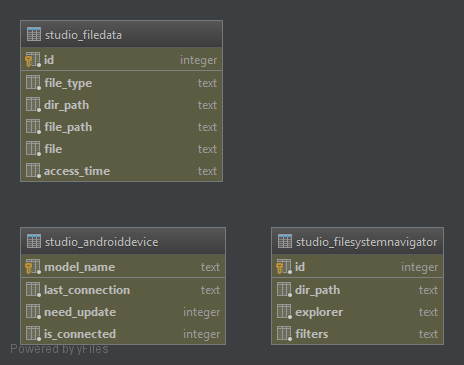
\includegraphics[scale=0.7]{djangodiagram.png}
\end{center}
\caption[Datos almacenados en \studio]{Datos almacenados en \studio}
\label{fig:djangodiagram}
\end{figure}